\documentclass[a4paper,12pt]{article} % тип документа

% report, book

% Рисунки
\usepackage{graphicx}
\usepackage{wrapfig}

\usepackage{hyperref}
\usepackage[rgb]{xcolor}
\hypersetup{				% Гиперссылки
    colorlinks=true,       	% false: ссылки в рамках
	urlcolor=blue          % на URL
}

%  Русский язык

\usepackage[T2A]{fontenc}			% кодировка
\usepackage[utf8]{inputenc}			% кодировка исходного текста
\usepackage[english,russian]{babel}	% локализация и переносы


% Математика
\usepackage{amsmath,amsfonts,amssymb,amsthm,mathtools} 


\usepackage{wasysym}

\author{Анна Назарчук Б02-109}
\title{1.2.3 Исследование взаимной диффузии газов}
\date{}
\begin{document}
\maketitle
\section{Аннотация}
Экспериментальное определение коэффициента взаимной диффузии с помощью датчиков теплопроводности при разных рабочих давлениях в системе и разных концентрациях газов. 
\section{Теоретические сведения}
Закон Фика:
\begin{equation}
j_a=-D\frac{\partial n_a}{\partial x}, j_b=-D\frac{\partial n_b}{\partial x}
\end{equation}
В опыте: диффузия гелия на стационарном воздухе:
\begin{equation}
D=\frac{1}{3}\lambda \bar{\upsilon}, \lambda = \frac{1}{n_0\sigma}, \bar{\upsilon} = \sqrt{\frac{8RT}{\pi \mu}}
\end{equation}
В общем случае:
\begin{equation}
D = \frac{1}{3}\lambda \bar{\upsilon}, \lambda = \frac{1}{n_{\Sigma}\sigma}, n_{\Sigma} = n_{He}+n_{\text{в}}=\frac{P}{kT}, \bar{\upsilon} = \sqrt{\frac{8kT}{\pi \bar{m}}}
\end{equation}
Следовательно, $D\sim \frac{1}{p}$
\section{Методика измерений}
\begin{figure}[h!]
\begin{center}
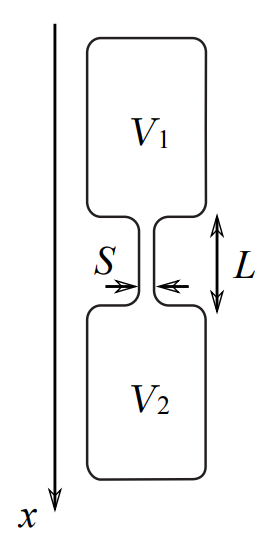
\includegraphics[width=0.3\textwidth]{Схема}
\end{center}
\caption{Схема используемых в измерении сосудов} \label{схема}
\end{figure}
\begin{equation}
V_1 \approx V_2\equiv V, LS\ll V \Rightarrow n(t)
\end{equation}
Через некоторое время в трубе (рис. \ref{схема})
\begin{equation}
j = -D\frac{\partial n}{\partial x} = const, n(x) = \frac{\Delta n}{L}x
\end{equation}
Для сосудов:
\begin{equation}
N_1=n_1V, N_2=n_2V, \frac{dN_1}{dt}=jS, \frac{dN_2}{dt}=-jS
\end{equation}
\begin{equation}
\frac{(d\Delta n)}{dt} =- \frac{\Delta n}{\tau}, \tau = \frac{1}{D}\frac{VL}{2S}
\end{equation}
\begin{equation}
\Delta n = \Delta n_0 e^{-\frac{t}{\tau}}
\end{equation}
Применимость: 
\begin{equation}
\tau \gg \tau_{\text{диф}}=\frac{L^2}{2D}, \Rightarrow SL\ll V
\end{equation}
\begin{figure}[h!]
\begin{center}
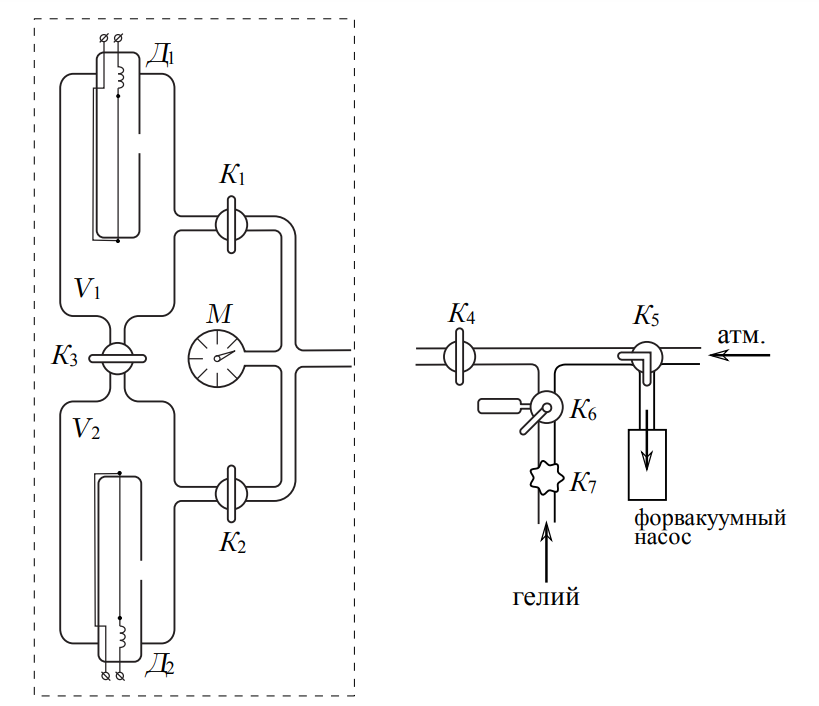
\includegraphics[width=0.6\textwidth]{Трубы}
\end{center}
\caption{Схема используемой в измерении установки} \label{трубы}
\end{figure}

Для теплопроводности (датчики в установке \ref{трубы})
\begin{equation}
\Delta k = k(n_2)-k(n_1)\approx const\cdot \Delta n
\end{equation}
Измерение разности теплопроводности с помощью измерения напряжения на гальванометре на мосту: при одной смеси в сосудах - баланс, при разных:
\begin{equation}
U\sim \delta k \sim \Delta n, U = U_0\cdot e^{-\frac{t}{\tau}}
\end{equation}
\section{Используемое оборудование}
Используемое оборудование в работе:
измерительная установка, форвакуумный насос, баллон с газом,  манометр, источник питания, магазин сопротивлений, компьютер.
Схема установки представлена на рис. \ref{трубы}, \ref{схема}, \ref{мост}, \ref{дозатор}
\begin{figure}[h!]
\begin{center}
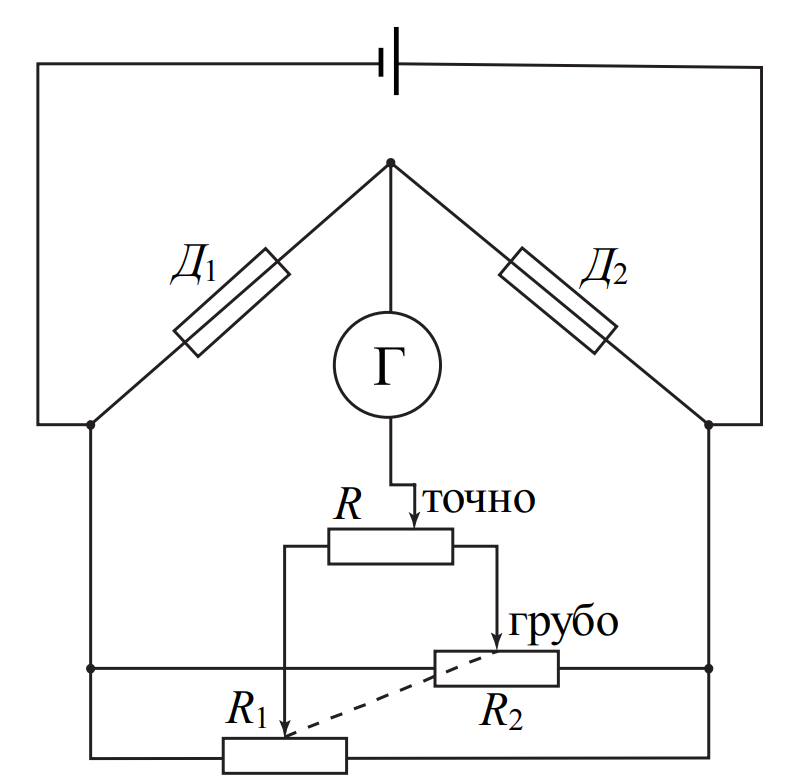
\includegraphics[width=0.4\textwidth]{Мост}
\end{center}
\caption{Схема используемого в измерении моста} \label{мост}
\end{figure}
\begin{figure}[h!]
\begin{center}
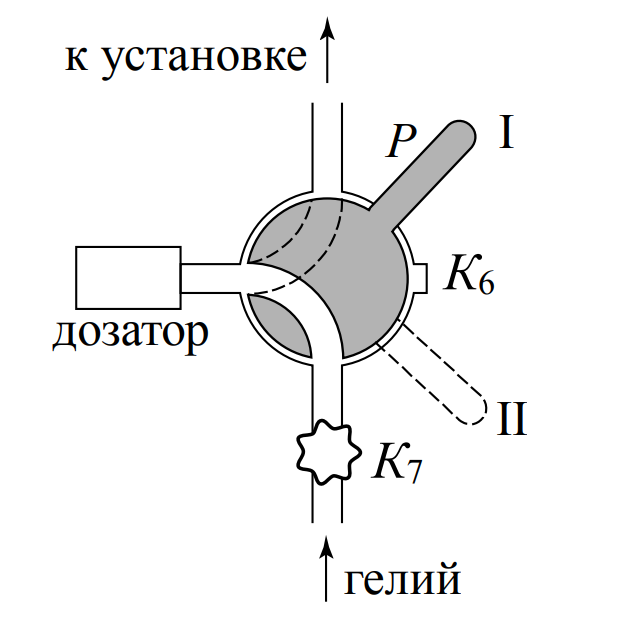
\includegraphics[width=0.3\textwidth]{Дозатор}
\end{center}
\caption{Схема используемого в измерении дозатора} \label{дозатор}
\end{figure}
Мост включает в себя датчики теплопроводности, гальванометр и переменное споротивление для балансировки моста.
Погрешности приборов указаны в таблице \ref{погрешности}
\begin{table} \label{погрешности} \caption{Погрешности приборов}
\begin{tabular}{|c|c|c|}
\hline 
Прибор & Гальванометр & Манометр \\ 
\hline 
Погрешность & 2,5\%  & 0.5 дел = 3.8 торр \\ 
\hline 
\end{tabular} 
\end{table}

\section{Обработка данных}
Постоянные характеристики устнаовки предствалены в таблице \ref{const}
\begin{table} \label{const} \caption{Постоянные параметры установки}
\begin{tabular}{|c|c|c|}
\hline 
L/S, 1/$\text{см}^2$ & V, $\text{см}^3$ & p0, торр \\ 
\hline 
$ 5.5 \pm 0.5$ & $1200 \pm 30$ & $756.2 \pm 3.8$ \\ 
\hline 
\end{tabular} 
\end{table}
Рассморим сначала диффузию гелия на стационарном воздухе.
Из измерений получили зависимость напряжения на гальванометре от времени при разных рабочих давлений. Результаты измерений представлены в виде графиков (рис. \ref{u1}, \ref{u2}, \ref{u3}, \ref{u4}), масштаб логарифмический.

\begin{figure}[h!]
\begin{center}
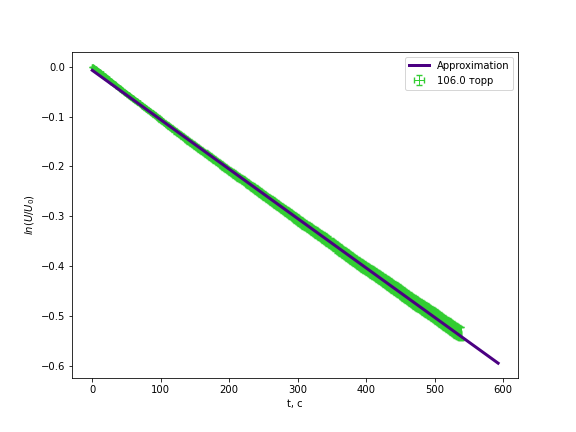
\includegraphics[width=0.8\textwidth]{U(t)+10}
\end{center}
\caption{Зависимость напряжения от времени при $p=106$ торр} \label{u1}
\end{figure}

\begin{figure}[h!]
\begin{center}
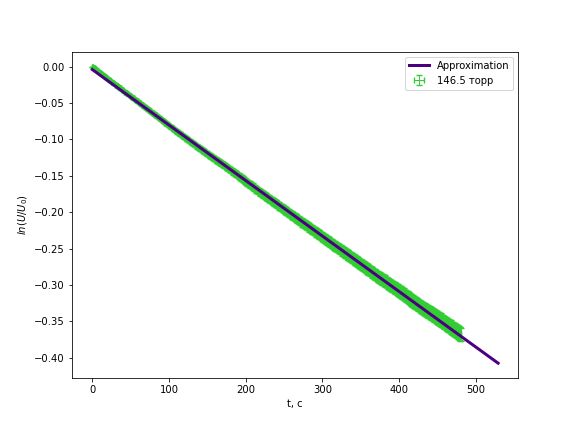
\includegraphics[width=0.8\textwidth]{U(t)+14}
\end{center}
\caption{Зависимость напряжения от времени при $p=146.5$ торр} \label{u2}
\end{figure}

\begin{figure}[h!]
\begin{center}
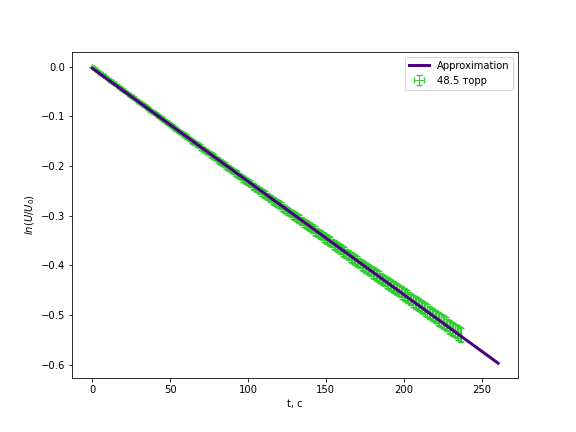
\includegraphics[width=0.8\textwidth]{U(t)+48}
\end{center}
\caption{Зависимость напряжения от времени при $p=48.5$ торр} \label{u3}
\end{figure}

\begin{figure}[h!]
\begin{center}
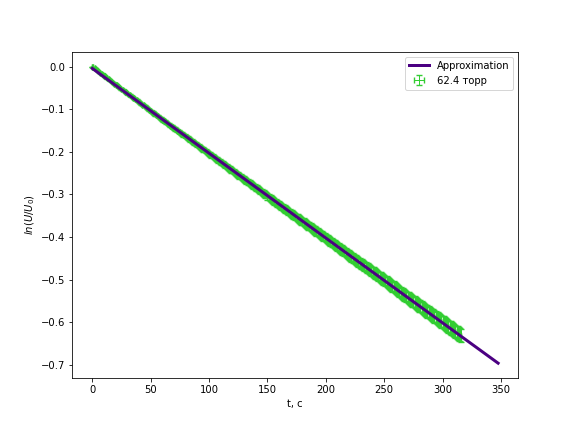
\includegraphics[width=0.8\textwidth]{U(t)+62}
\end{center}
\caption{Зависимость напряжения от времени при $p=62.4$ торр} \label{u4}
\end{figure}

Для каждого давления посчитаем D:
\begin{equation}
D = -\frac{kVL}{2S}
\end{equation}
k - угловой коэффициент наклона графика.

И погрешность D:
\begin{equation}
\sigma_D = D\cdot \sqrt{(\frac{\sigma_k}{k})^2+(\frac{\sigma_V}{V})^2+(\frac{\sigma_{L/S}}{{L/S}})^2}
\end{equation}
Наибольший вклад в погрешность вносит погрешность отношения $L/S$
Результаты в таблице \ref{D}

\begin{table} \label{D} \caption{Значения коэффициента взаимной диффузии при разных давлениях} \begin{tabular}{|c|c|c|} \hline D, $sm^2/s$&	$\sigma_D$, $sm^2/s$ & p, торр \\ \hline 6.571 & 0.62 & 62.4 \\ \hline 3.27 & 0.308 & 106.0 \\ \hline 2.517 & 0.237 & 146.5 \\ \hline 7.515 & 0.709 & 48.5 \\ \hline \end{tabular} \end{table}
Представим данные из таблице в виде графика зависимости D от 1/p (рис. \ref{D_p})

\begin{figure}[h!]
\begin{center}
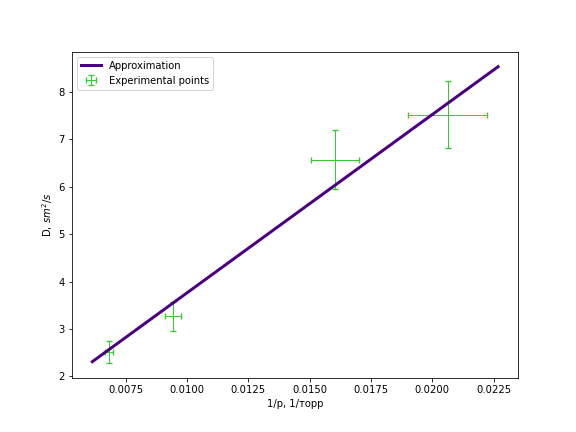
\includegraphics[width=0.8\textwidth]{D(p)}
\end{center}
\caption{Зависимость коэффициента взаимной диффузии от давления} \label{D_p}
\end{figure}

Найдем угловой коэффициент наклона прямой на графике, расчитаем значение D при атмосферном давлении:
\begin{equation}
k = 376.2 \pm 11.6 sm^2/s/\text{торр}
\end{equation}
Погрешность коэффицента взаимной диффузии при атмсферном давлении:
\begin{equation}
\sigma_{D(p_0)}=D(p_0)\cdot \sqrt{(\frac{\sigma_k}{k})^2
+(\frac{\sigma_{p_0}}{p_0})^2}
\end{equation}
Вклад слагаемых в погрешность примерно одного порядка.
\begin{equation}
D(p0)=k/p0=0.51 \pm 0.02 sm^2/s
\end{equation} 
Табличное значение $D(p0) = 0.62 sm^2/s$, полученное значение близко к табличному.

Теперь рассмотрим диффузию примеси воздуха с гелием. Экспериментально получим зависимость напряжения на гальванометре (логарифмический масштаб) от времени, результат в виде графика (рис. \ref{u5})

\begin{figure}[h!]
\begin{center}
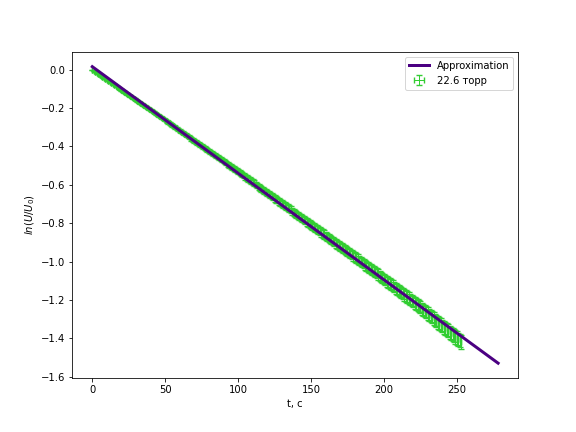
\includegraphics[width=0.8\textwidth]{U(t)+22}
\end{center}
\caption{Зависимость напряжения от времени при $p=22.6$ торр} \label{u5}
\end{figure}
Посчитав угловой коэффицент (D), расчитаем D(p0) исходя из этих экспериментальных данных:
\begin{equation}
\sigma_{D(p_0)}=D_{p_0}\cdot \sqrt{(\frac{\sigma_D}{D})^2+(\frac{\sigma_p}{p})^2+(\frac{\sigma_{p_0}}{p_0})^2}
\end{equation}
\begin{equation}
D(p0)=D/p*p0 = 0.55 \pm 0.09 sm^2/s
\end{equation}
Можно заметить, что значения коэффициента взаимной диффузии данных газов при атмосферном давлении близки к друг другу, что свидетельствует о независимости коэффициента взаимной диффузии газов от начальных пропорций.

Посчитаем длину свободного пробега гелия в данных условиях:
\begin{equation}
\sigma_{\lambda_{He}} = \lambda_{He}\cdot \frac{\sigma_D}{D}
\end{equation}
\begin{equation}
\lambda_{He} = \frac{3D}{\bar{\upsilon}} = \frac{3D}{\sqrt{\frac{8RT}{\pi \mu}}}= ( 1.2 \pm 0.12 ) \cdot 10^{-7} \text{м}
\end{equation}

Из выражения для длины свободного пробега можно найти эффективное сечение столкновений атомов гелия с молекулами воздуха:
\begin{equation}
\sigma_\sigma = \sigma \sqrt{(\frac{\sigma_p}{p})^2+(\frac{\sigma_\lambda}{\lambda})^2}
\end{equation}
\begin{equation}
\sigma = \frac{1}{n_0\lambda} = \frac{kT}{p\lambda}= ( 3.4 \pm 0.3 ) \cdot 10^{-19} \text{м}^2
\end{equation}
Основоной вклад в данную погрешность дает неточность измерения давления.


\section{Вывод}
Получено значение коэффициента взаимной диффузии гелия и воздуха при разных пропорциях, видна идентичность полученных результатов при разных пропорциях газов и при сравнении с табличными значениями.
\end{document}